\subsection{Energy Utilization}


Unlike programming desktops, where one mainly 
  improves software by increasing either features or performance,
  mobile programmers develop for increase features, performance, and 
  battery life.
In fact, one of the main selling points for heterogeneous
  programming on mobile devices, is the increase in battery life.
Increasingly, hardware vendors, such as Apple or Samsung, sell new
  mobile hardware by advertising longer battery life.
Finding a balance between energy consumption and performance is a 
  balancing act that a programmer would like to delegate to the 
  compiler or runtime.


Since, mobile devices employ DVFS
  the energy utilization of the device at a specific time is governed by
  the operating frequency of the processor.
One can model~\cite{zhang2010accurate, dong2011self} the battery usage of the power draw at time $t$ by

\begin{align*}
P(t) &= \beta_v(\beta(t)) + G_u(t) ~ G_v(G_f(t)) \\
     &+ \sum_{i=1}^{N} C_{u_n}(t) ~ C_{v_n}(C_{f_n}(t))
\end{align*}

where $N$ the number of CPU cores, $\beta$ is the brightness of the LCD screen at time $t$, $\beta_v(br)$ is the power used for the specified brightness level, $G_f(t)$ and $C_{f_n}(t)$ are the operating frequencies at time $t$, and $G_v(f)$ and $ C_{v_n}(f)$ are the power draws for the processors at the specified voltage, $G_u(t)$ and $C_{u_n}(t)$ are the processor utilizations at time $t$.
Other terms, such as GPS, wireless, and other sensors, can be measured or modeled, but for this analysis we turn them off.

The issues with using a model is determining the the power draw at the specified
  frequency (which is not specified by the processor's manufacturer) and the method of reading
  the CPU and GPU counters is varies from device to device.
As a result, we again use Trepn to read the hardware counters giving us the battery usage (in $uW$) at each time interval.
Battery usage consists of all power-consuming components, e.g., screen, CPU, GPU, and memory.
If, for example, the computation takes longer then more power is consumed by other components, such as the screen.
Therefore, the energy consumed by a computation is not only dependent on of the load, but also the time it takes to perform a computation.
We place the device in airplane mode (to disable GPS, wireless, and other sensors) and disconnect the device from a power source to 
  collect the data.
Similar to the when measuring the processor utilization, we only consider the case where the kernel is executed many times.

\begin{figure}
  \centering

  \begin{subfigure}[b]{0.5\textwidth}
          \centering
          
\includegraphics[width=0.6\textwidth]{data/legend.pdf}
  \end{subfigure}

  \begin{subfigure}[b]{0.23\textwidth}
      \centering
      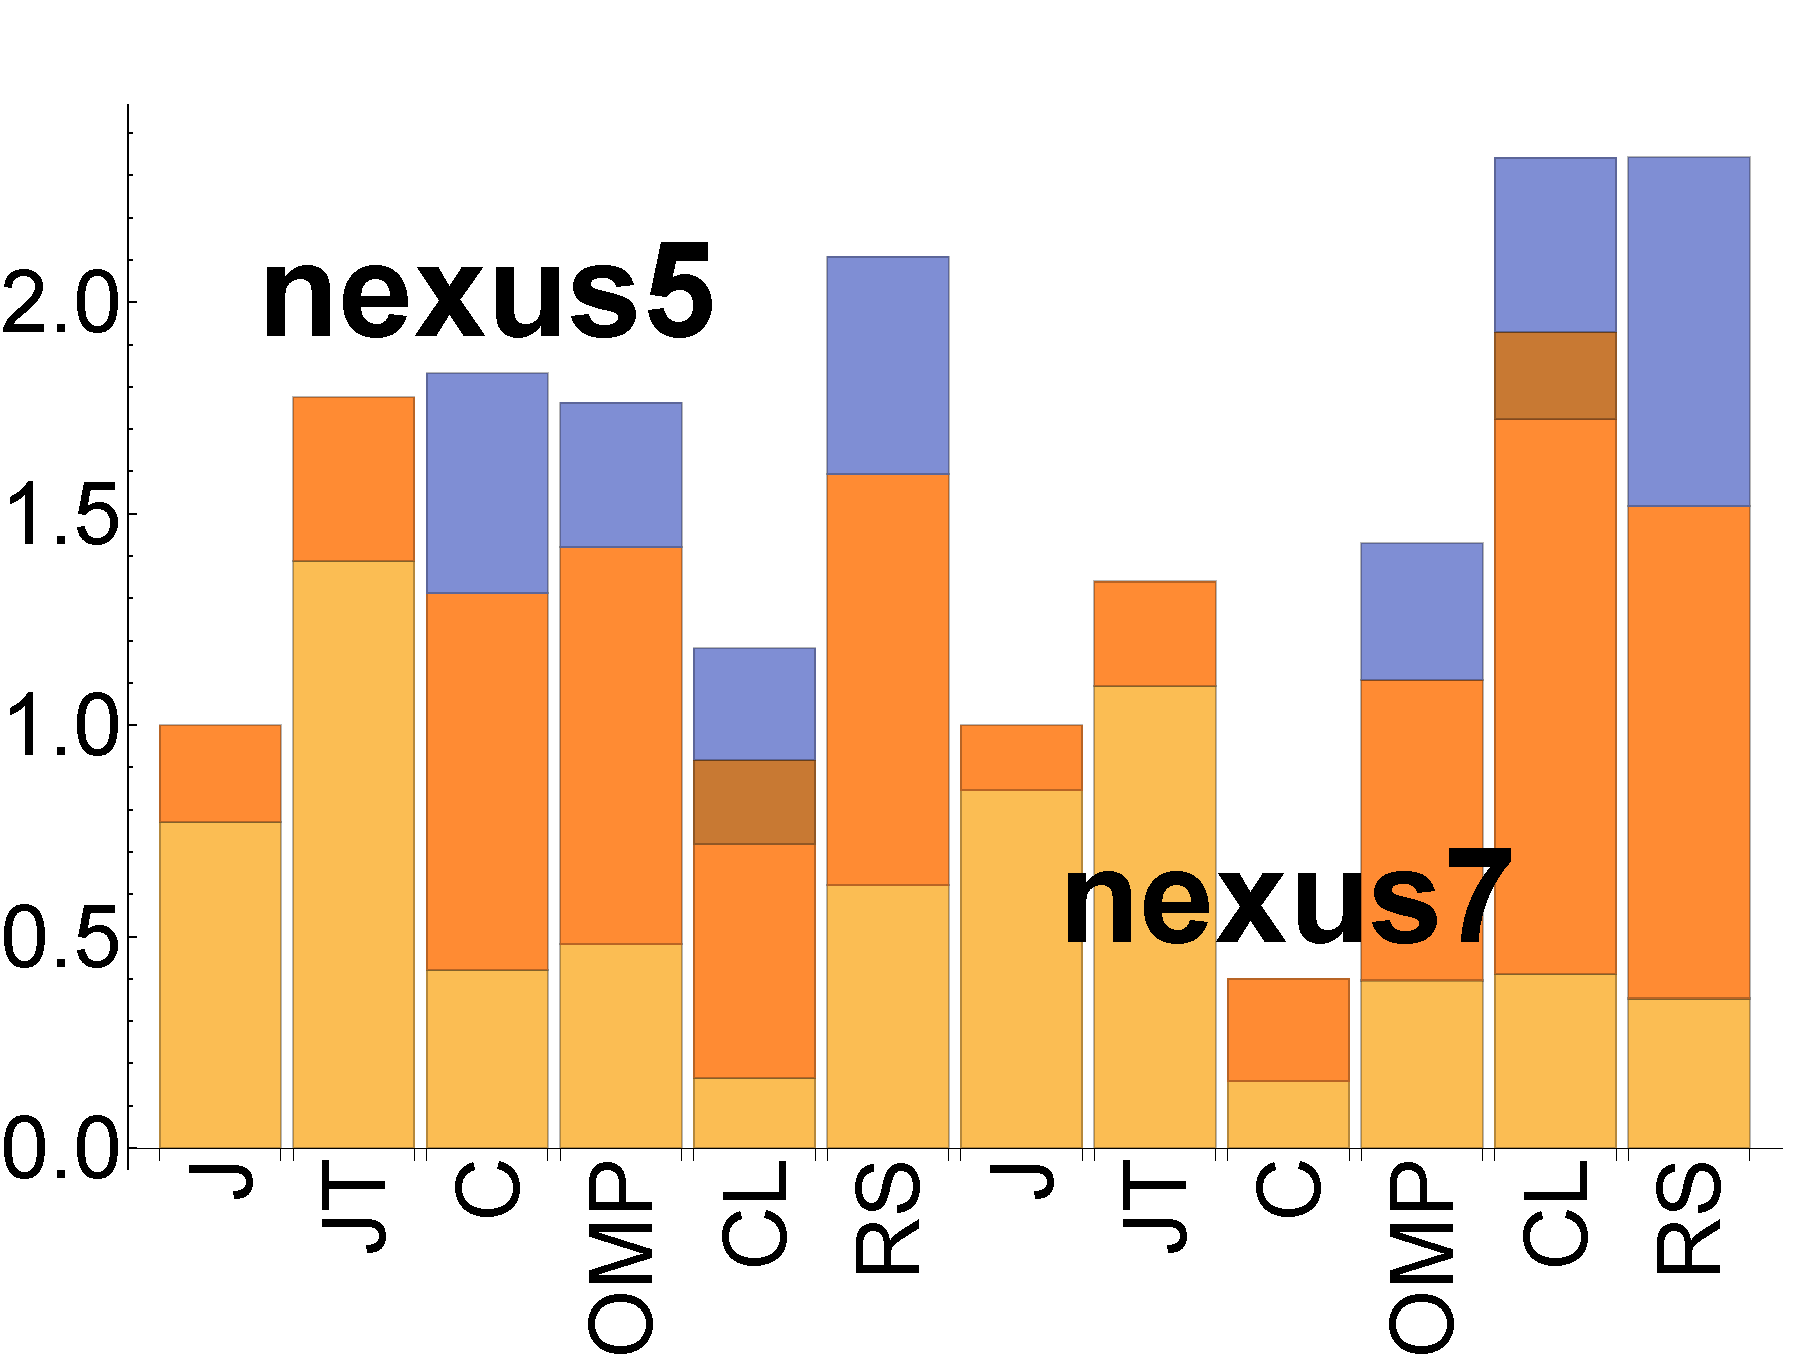
\includegraphics[width=0.9\textwidth]{data/bbattery_vectoradd.pdf}
      \caption{VectorAdd}
  \end{subfigure}%
  \begin{subfigure}[b]{0.23\textwidth}
      \centering
      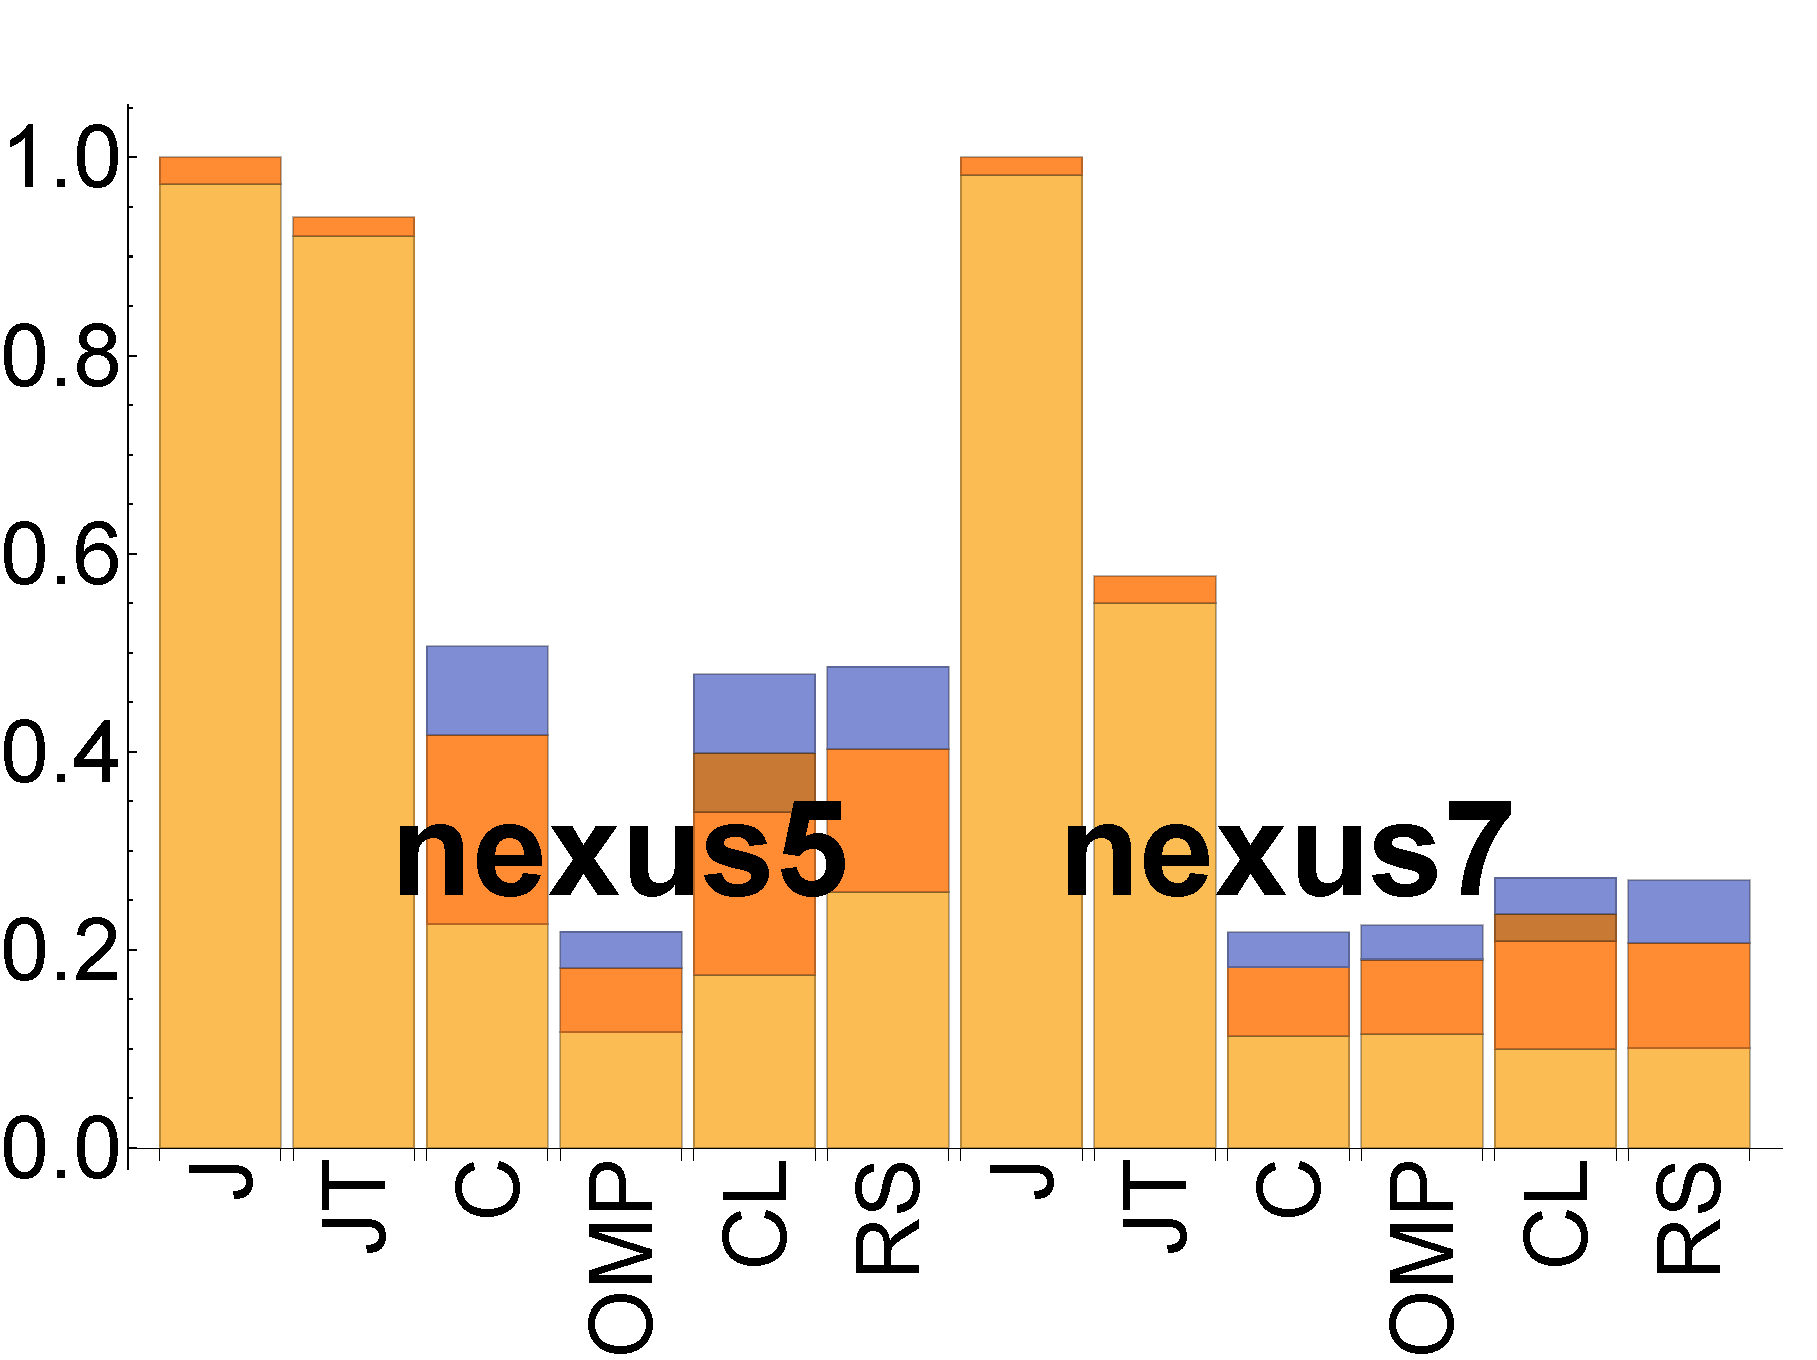
\includegraphics[width=0.9\textwidth]{data/bbattery_sgemm.pdf}
      \caption{Sgemm}
  \end{subfigure}


  \begin{subfigure}[b]{0.23\textwidth}
      \centering
      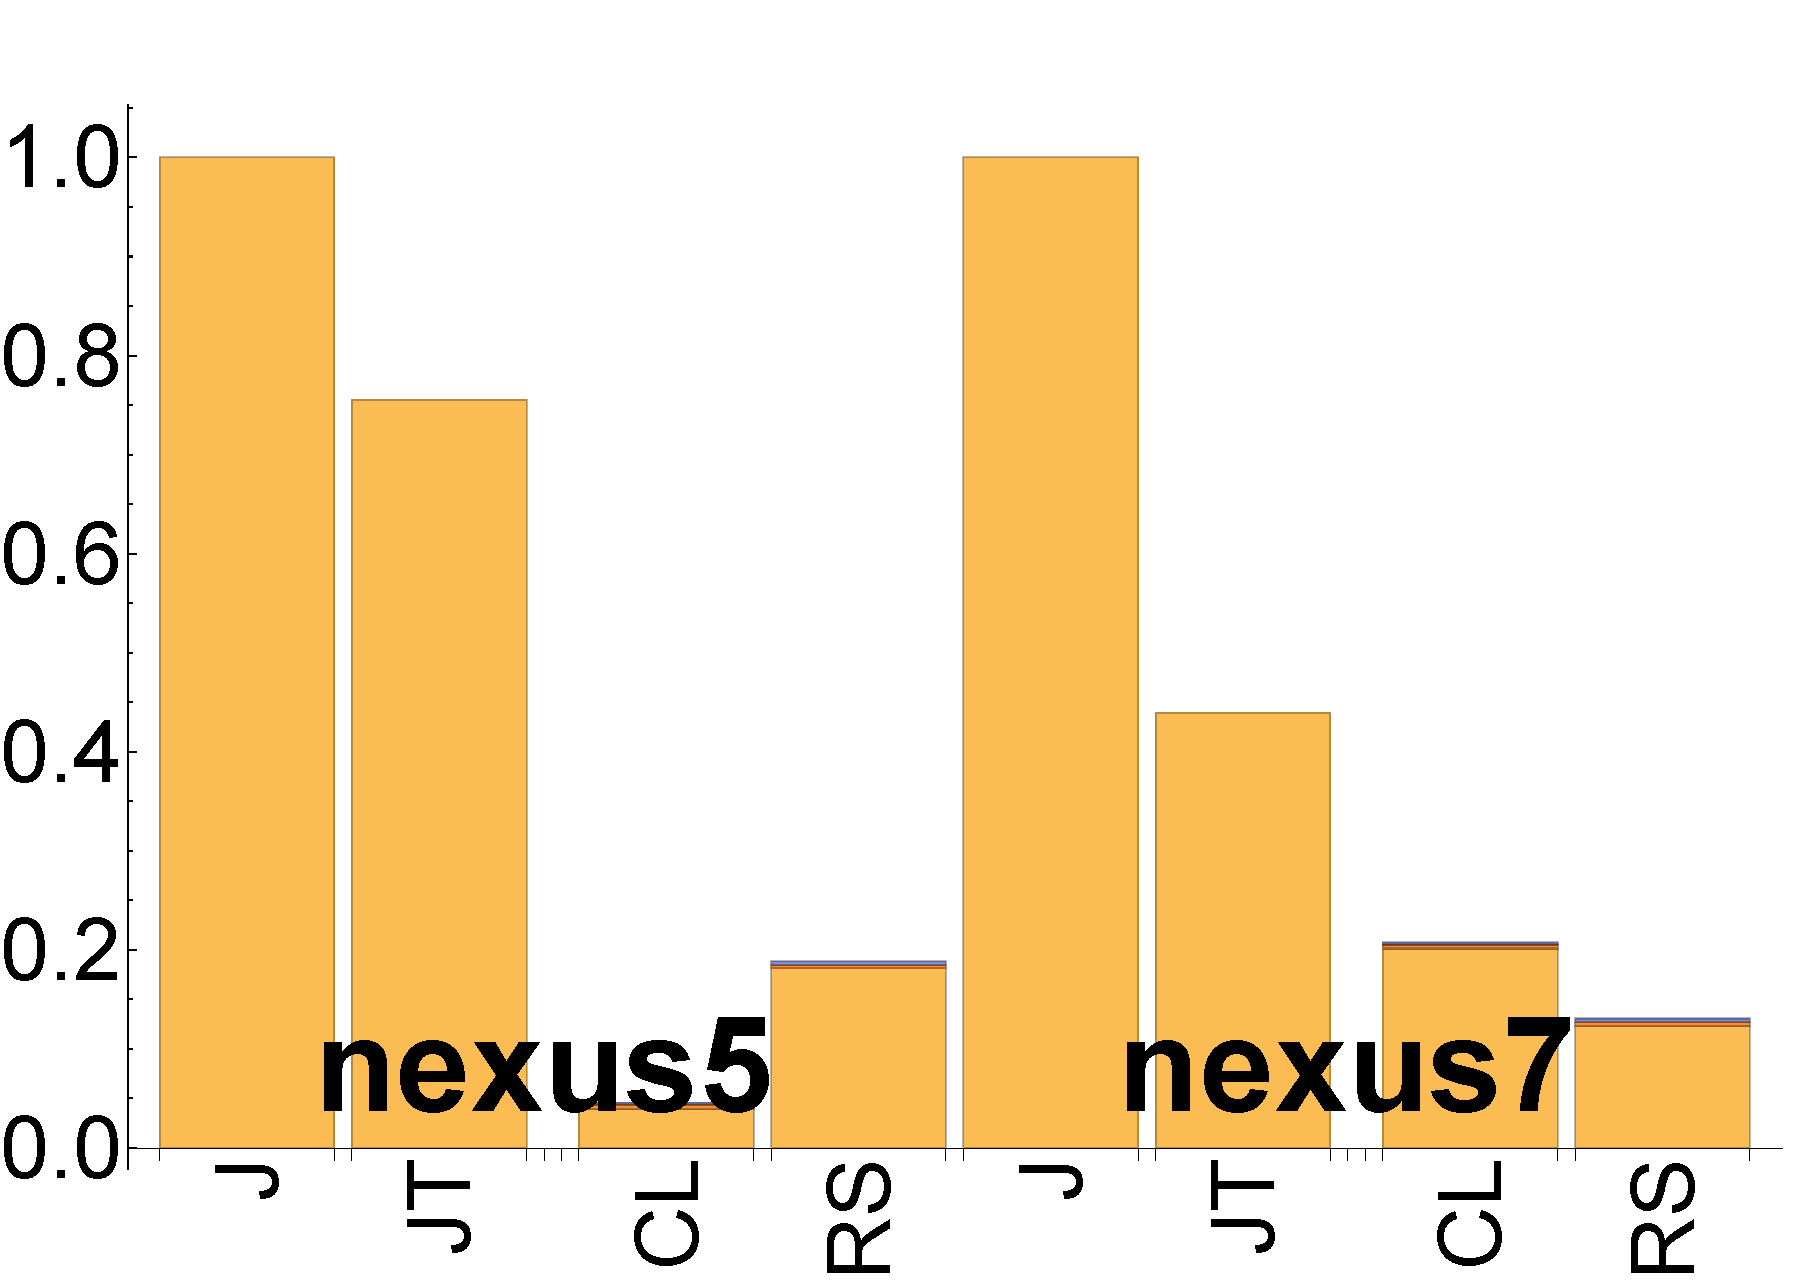
\includegraphics[width=0.9\textwidth]{data/bbattery_mriq.pdf}
      \caption{MRIQ}
  \end{subfigure}
  \begin{subfigure}[b]{0.23\textwidth}
      \centering
      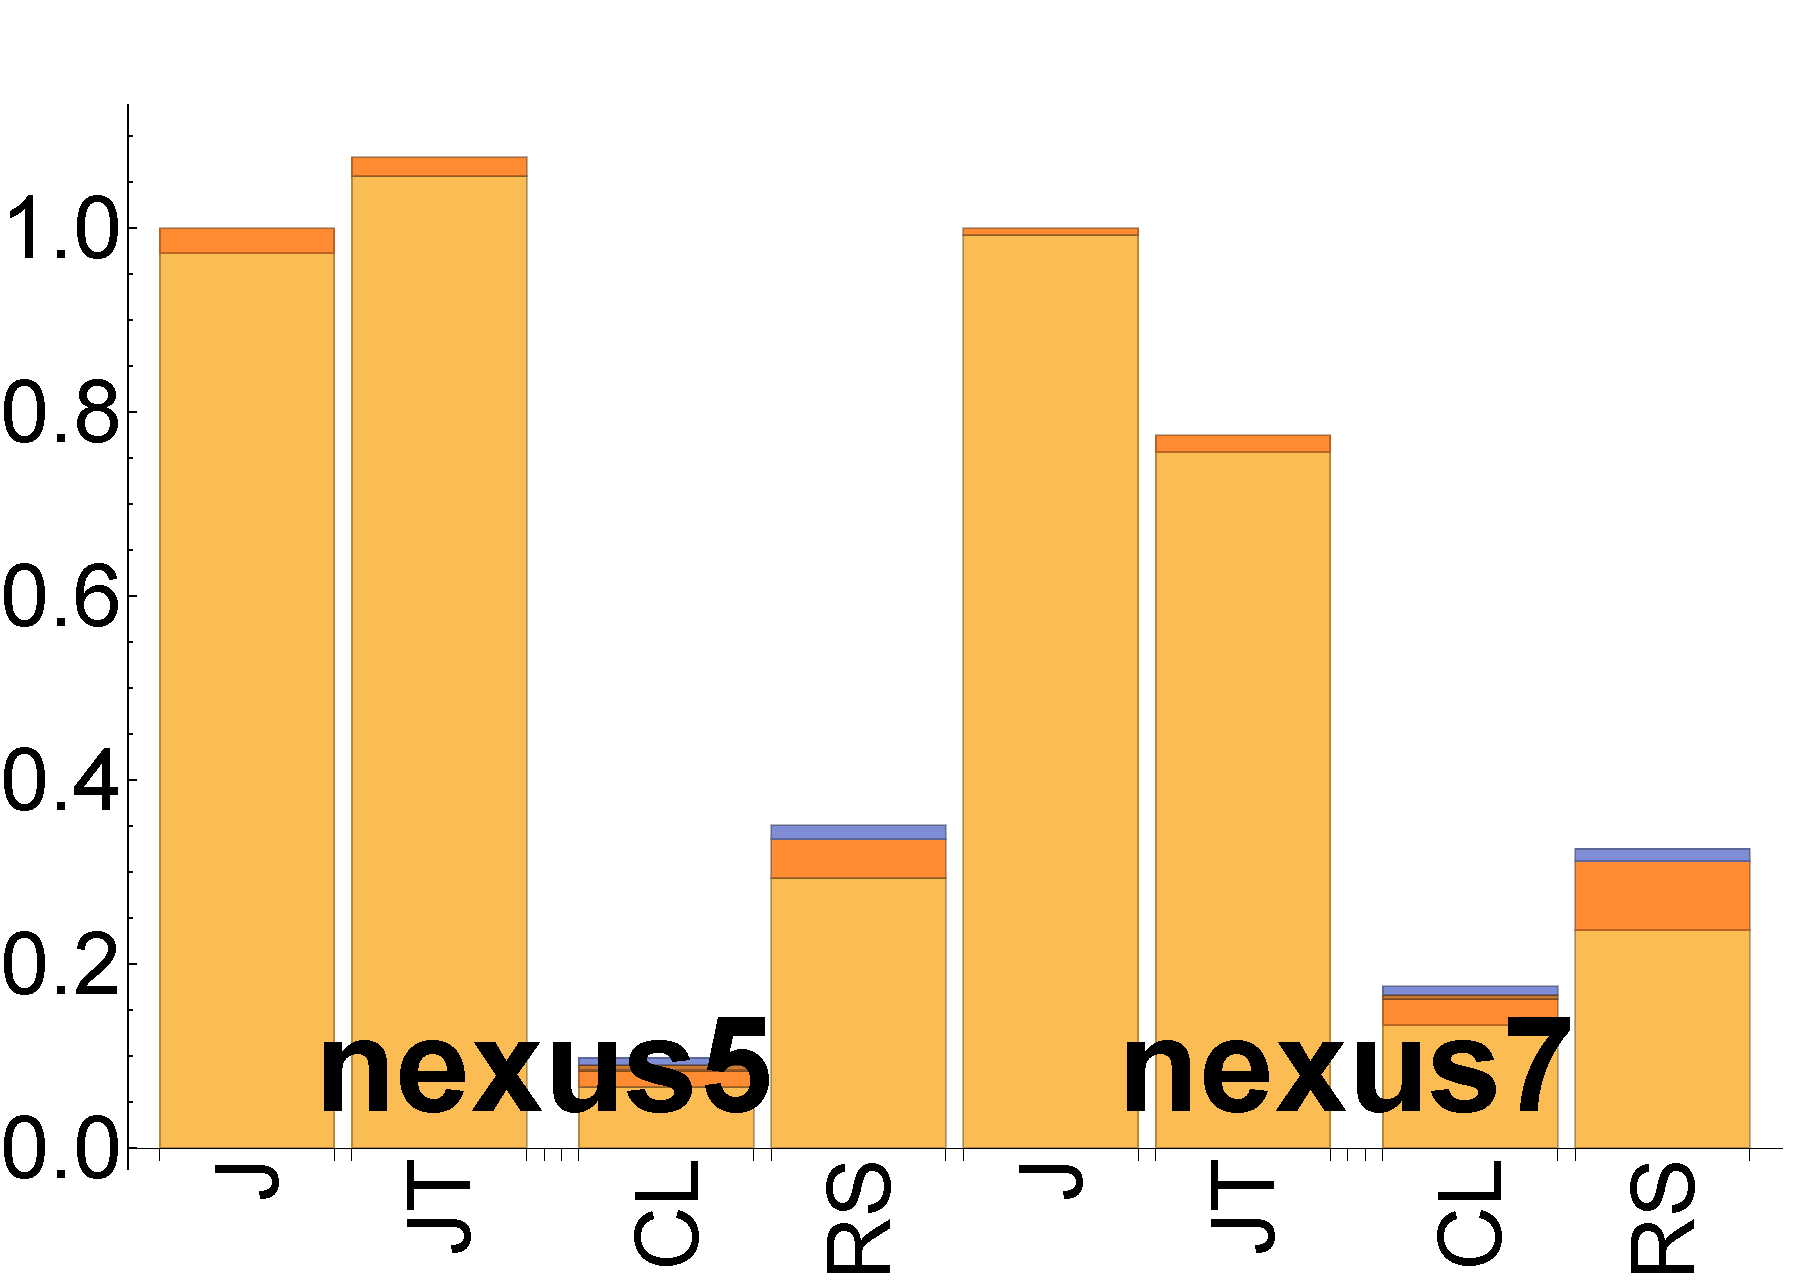
\includegraphics[width=0.9\textwidth]{data/bbattery_tpacf.pdf}
      \caption{TPACF}
  \end{subfigure}%

  \begin{subfigure}[b]{0.23\textwidth}
      \centering
      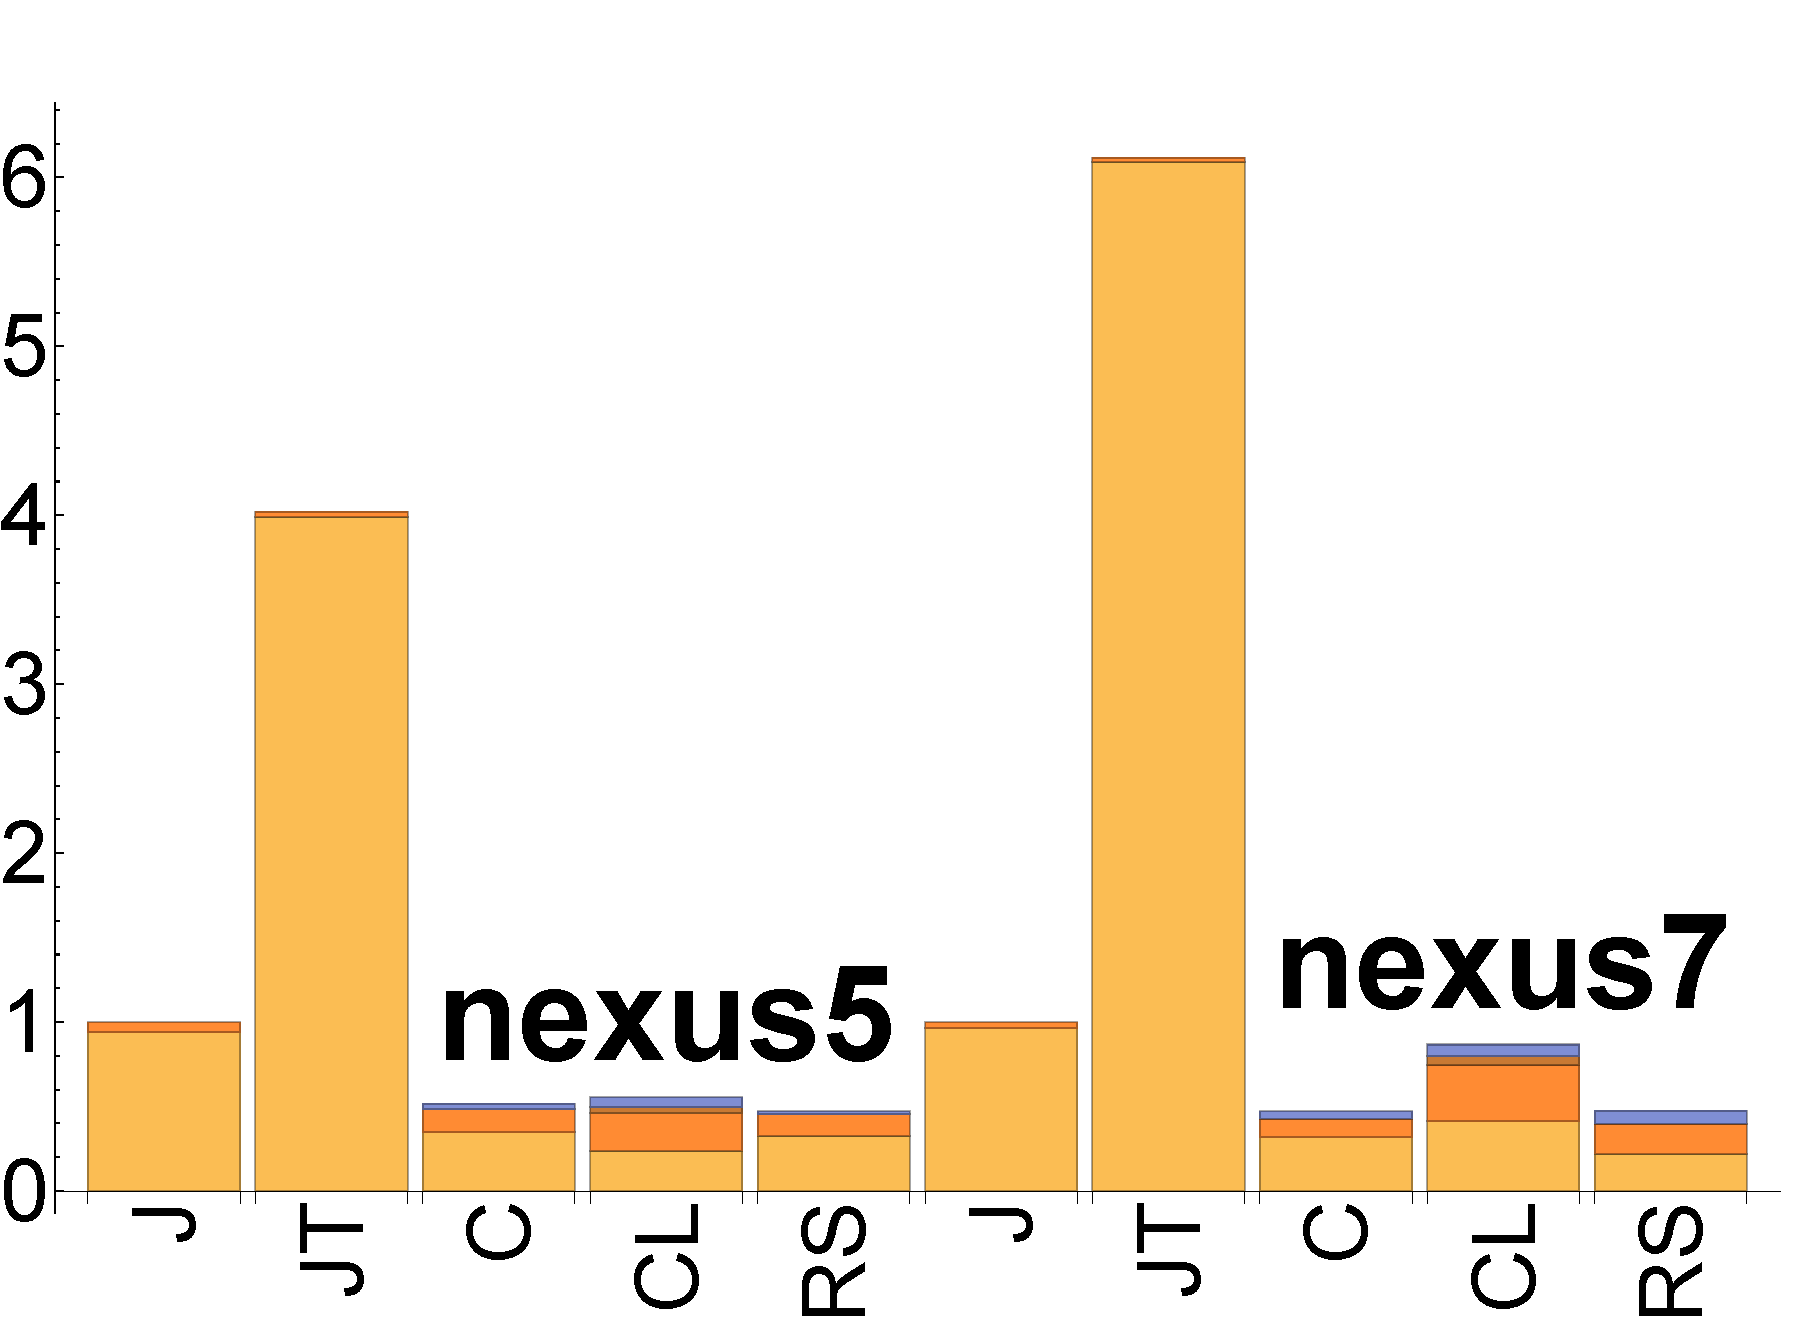
\includegraphics[width=0.9\textwidth]{data/bbattery_histogram.pdf}
      \caption{Histogram}
  \end{subfigure}%
  \begin{subfigure}[b]{0.23\textwidth}
      \centering
      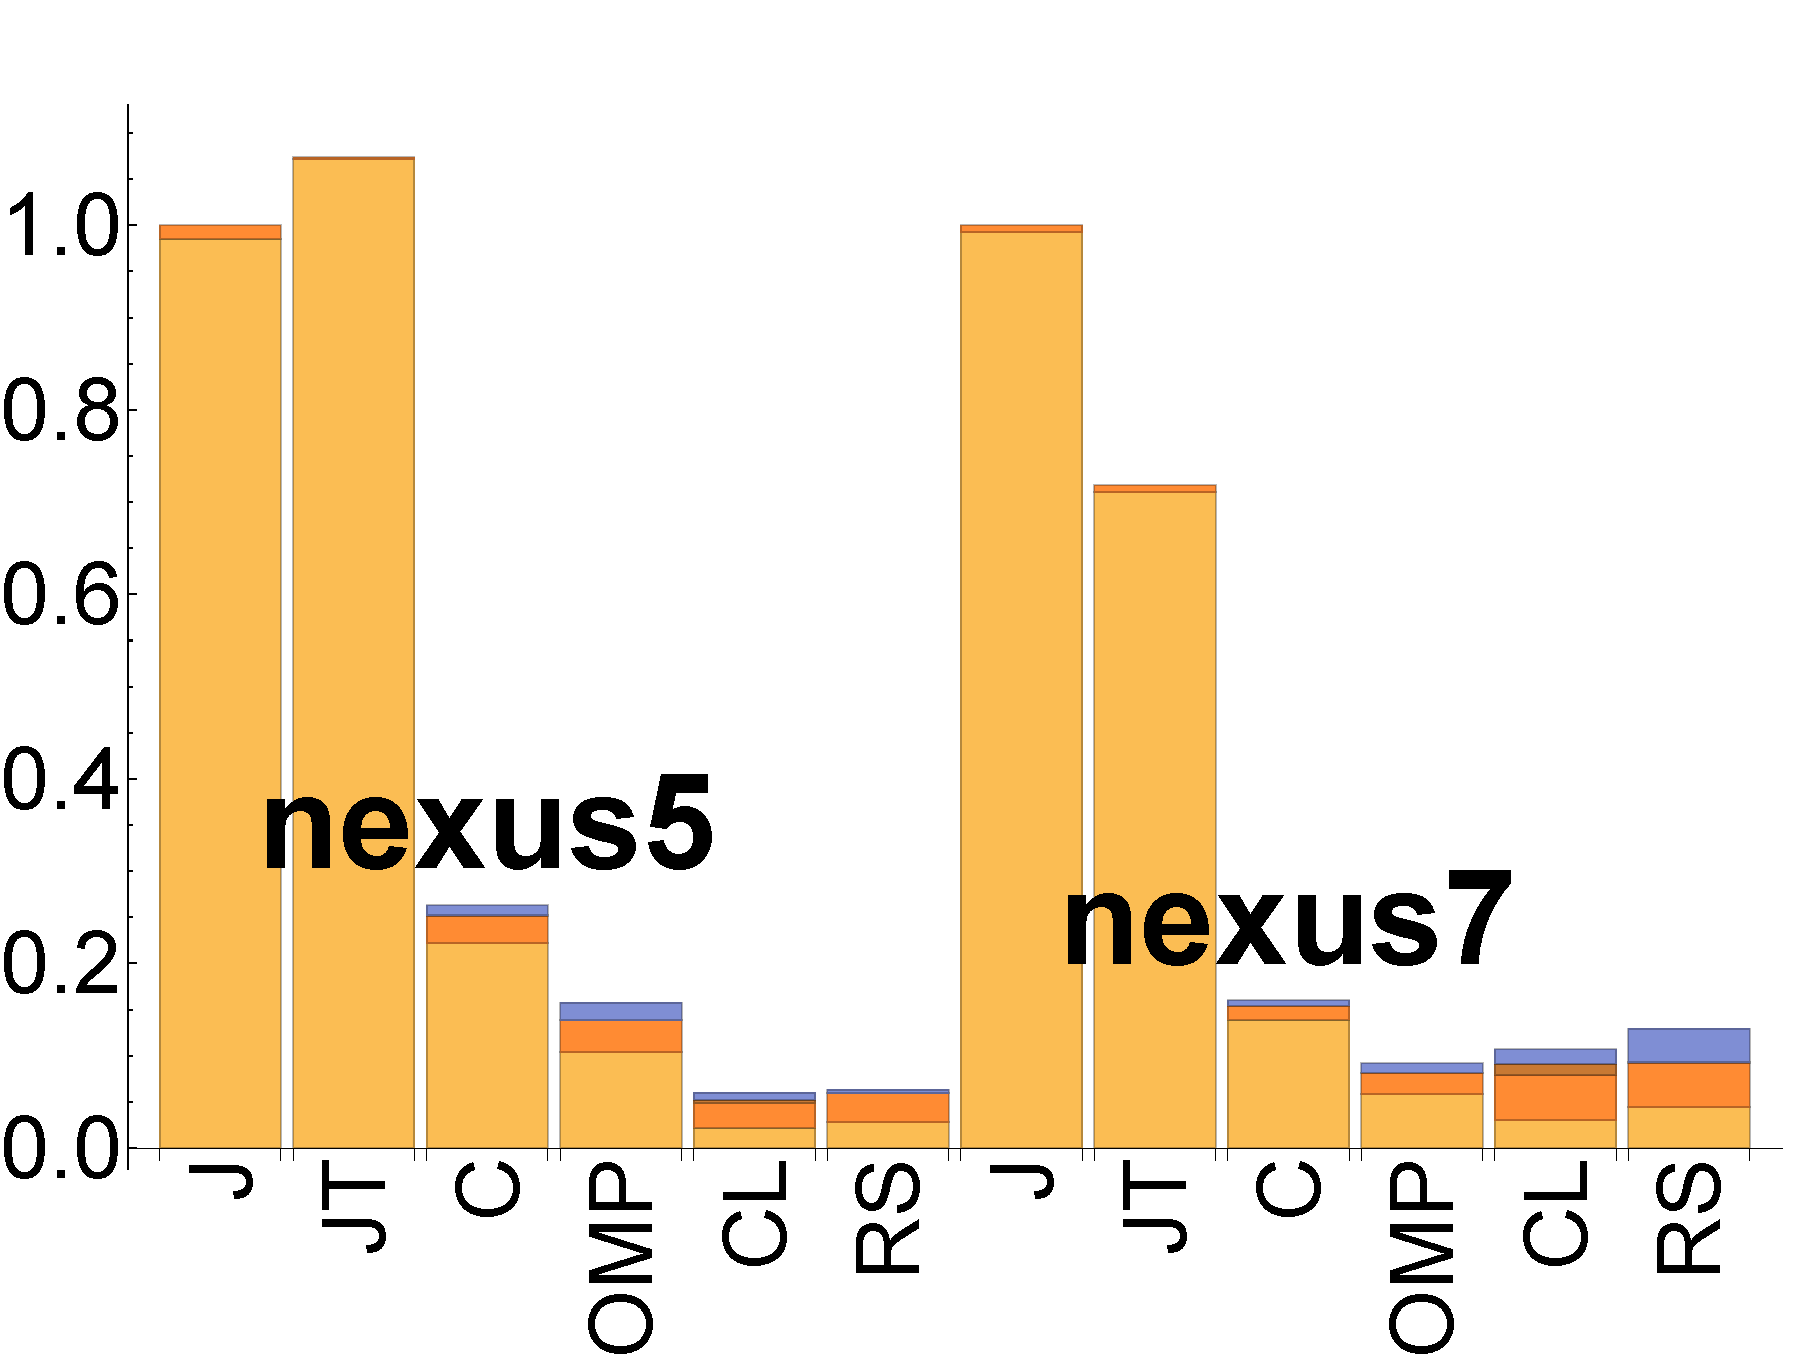
\includegraphics[width=0.9\textwidth]{data/bbattery_stencil.pdf}
      \caption{Stencil} 
  \end{subfigure}
  \caption{Energy usage for both the Nexus 5 and Nexus 7 normalized to Java's energy utilization (lower is better).}
  \label{fig:power}
\end{figure}

Figure~\ref{fig:power} shows the energy consumed by each implementation for both Nexus 5 and Nexus 7 
  (Trepn is not able to read hardware counters for the other devices).
While, as discussed in the previous section, RenderScript performs better, it does make full utilization of all CPU
  cores.
OpenCL, on the other hand, does not make use of all cores and only fully utilize the GPU.
Since OpenCL has a similar time profile as RenderScript on the Nexus 5, we observe that it is more energy efficient
  compared to RenderScript.
For the Nexus 7, some benchmarks RenderScript has better energy utilization while OpenCL is better in others.

Therefore, which implementation to choose to reduce energy consumption is device and compute pattern dependent.
Compared to the other implementations, RenderScript has lower energy consumption for any of the benchmarks.
It is also clear that the LCD screen makes a big impact on power usage, in MRIQ, for example, even though the threaded Java code
  utilizes all the CPU cores, because it is able to complete quicker it uses less power overall compared to the serial Java code.

